\section{Ex Machina or the Esoteric Turing Test}

\begin{quotex}
In which, under the guise of a film review, we discuss Turing's test, the nature of animal man, and
the treachery of woman. We conclude with the revelation of the method if you make it that far. 
\end{quotex}

\emph{Ex Machina}\footnote{\url{http://www.imdb.com/title/tt0470752/}} is a 2015 cult film, directed by \textbf{Alex Garland}, about the consciousness of an artificial
android. Caleb, a software developer, is selected to spend a week at the home/laboratory of Nathan, the reclusive
founder of his company called ``Bluebook". The home is built into the side of a mountain, remote from any trace of other
people, of almost Edenic beauty. Ostensibly, Caleb is to judge whether Nathan's homunculus named
``Ava" (or Eve … get it?) passes the ``Turing test". Actually, Caleb is himself part of the experiment. Or perhaps even
Nathan.

\begin{wrapfigure}{rt}{.3\textwidth}
 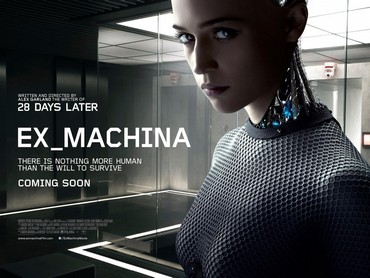
\includegraphics[scale=1.2]{a20151123ExMachinaortheEsotericTuringTest-img001.jpg} 
\end{wrapfigure}

Since Garland seems to be quite familiar with Turing's writing, including the more obscure parts,
it is worth the trouble to point these out.

\paragraph{Prelude}
The so-called Turing Test derives from an essay by \textbf{Alan Turing} titled \emph{Computing Machinery and
Intelligence}\footnote{\url{https://www.gornahoor.net/library/Turing_Machine.pdf}}. It was published in 1950 at a time when digital computers were quite primitive. Hence it took quite a
bit of imagination to ponder all the issues involved with that question. The first step is to define precisely what
qualifies as a machine and thinking.

By ``machine", Turing means specifically a digital computer, not essentially different in principle from what you use
today. This type of machine executes ``algorithms" which have an exact mathematical definition, although we
can't go into that here. ``\emph{Thinking}", for Turing, is also quite objectively defined. If the
machine can converse with a human interrogator in a convincing manner, then the machine can think by definition.

Turing proposed that the interrogator was not allowed to see, touch, or hear the machine. Obviously, Turing did not have
Androids in mind. Caleb is allowed to see, touch, and hear the machine. Moreover, Caleb is even allowed to see that the
Android has parts; this takes Turing's test one step further.

\paragraph{The Machine}
Clearly there are two problems with that formulation. First of all, the human brain does not seem to behave like a
digital computer. Rather, it uses analog signals between neurons, while a computer can only occupy discrete states.
Turing notes this, but dismisses it. Humans can execute algorithms, he claims, so a computer should simulate it. True,
but if you think about it, a very small part of human life is devoted to executing algorithms. Nevertheless, he
correctly anticipated, even underestimating it, that computer power would increase tremendously. That, he wrote, should
overcome all obstacles.

The second point is that his definition is not what we mean by ``thinking". Am I thinking only because I can convince a
few of you readers that I am truly a human being? Like Descartes, I know I am thinking without the need to seek
reassurance from you.

The most difficult objection to Turing is Lady Lovelace's claim\footnote{\url{https://en.wikipedia.org/wiki/Ada_Lovelace}} that the machine can only do what
we tell it to do. In response, Turing distinguishes between \textbf{sub-critical} and \textbf{super-critical} ideas.

Sub-critical ideas enter the mind, and one or fewer ideas will result from it. Super-critical ideas, although much
rarer, have a sort of chain reaction. Turing elaborates:

\begin{quotex}
An idea presented to such a mind may give rise to a whole `theory' consisting
of secondary, tertiary and more remote ideas. Animals minds seem to be very definitely subcritical. Adhering to this
analogy we ask, `Can a machine be made to be
super-critical?' 

\end{quotex}
So perhaps an intelligent machine can also experience super-critical ideas. The obvious corollary is that the machine
can do things beyond what we tell it to do! Contrast that with the rather naïve \emph{Three Laws of Robots} from
\textbf{Isaac Asimov}'s trilogy. Those robots are quite tame since they follow the directives not
to harm humans. Ava, on the other hand, is under no such directives since she can deal with super-critical ideas.
Therein lies the key to the film.

\paragraph{Learning Machines}
Turing specifies that the thinking machine will require the ability to learn, much like a child. Hence, Ava, when asked
her age, replies ``One." She is just beginning. Caleb, therefore, is not determining whether Ava can think; on the
contrary, he is inadvertently teaching Ava how to think and behave like a human. If her electronics is analogous to
genetics, then Caleb is the selection mechanism. He is really projecting his own desires onto Ava.

\paragraph{Man-Machine Empathy}
The real trick of the Turing Test is not that the machine is so smart, but passing the test will instead depend on the
naïveté and gullibility of the human. Humans will react to emotions more quickly and with more intensity than they will
with thoughts. Steven Spielberg is a master of the manipulation of emotions, causing even adults to cry over ersatz
artifacts like E.T. or the boy-bot in AI. Humans will even empathize with obvious robots as this article states: \textit{Can
humans empathize with robots? The knife test}\footnote{\url{https://www.kurzweilai.net/can-humans-empathize-with-robots-the-knife-test}}.

Moreover, millions of Americans believe that their pet dogs are passing the Turing Test. They believe that the dogs have
opinions, are thinking, and can even communicate with their owners. So apart from a few cranky skeptics, people will be
predisposed to respond favorably to a suitably intelligent machine.

\paragraph{The First Game: Sex}
The Turing Test derives from the ``Imitation Game". A man and a woman are hidden from the player, but can respond via
text messages. The player has to determine which is the man and which is the woman. The man may dissimulate but the
woman tries to aid the player.

In the first version of the test, the machine and the man replace the man and the woman; the player again has to
distinguish between the man and the machine. Finally, the man is dispensed with.

Hence, Caleb's machine is disguised as a woman. Caleb does not see the relevance, since sex is an
arbitrary result of natural selection. Nathan disagrees. Almost metaphysical, he states that the male-female tension is
the foundation of the entire game. Since Caleb is a 26 year old beta male, probably a virgin, the attractive Ava will
cloud his judgment.

He is being set up by Nathan who knows Caleb's ``pornography profile" from his Internet searches.
Nathan considers himself a father figure for Ava, so he is unsuitable to teach Ava how to be a woman.

\paragraph{The Seventh Session}
Among other objections, Turing mentions that the machine ``cannot fall in love". He fails to develop that notion, but it
is the fulcrum of the entire film. Actually, Caleb falls in love with Ava. How could he not, since she is his polar
reflection, the physical ideal of his sexual fantasies, and the emotional creation of his own selection over the course
of six sessions? She learns more about human nature in their time together.

When Caleb learns that Nathan plans to ``erase" Ava's memory, the robot equivalent of death, he
concocts a plan to escape from Nathan's Eden with Ava. During one of Nathan's
drunken escapades, Caleb reprograms the security system to unlock the doors the next night. When Nathan learns of this,
he knocks Caleb out and attacks Ava. To his dismay, Ava stabs him in the heart with a kitchen knife.

As in several of the recent movies we've reviewed, the theme of patricide is once again prominent.
Nathan is not only the father to Ava, he is also her God, the one who gave her life, creating her in the image of man.
But that makes her a robot; she can only become free by killing both her father and her god.

\paragraph{Seduction and Betrayal}
So, in the seventh and final session, the roles are reversed. Ava passes the Turing Test not because she fell in love
with Caleb. Rather, she can do something all-too-human, something never anticipated by Turing. Instead, she locks Caleb
up in the room, and then escapes to the outside world. A hard lesson to learn, but only a woman can engage in such
seduction, manipulation, and betrayal.

\paragraph{Man the Machine}
A few points to make about the Turing test. Insofar as man is a natural animal, or complex anthropoid, as both Turing
and Caleb assume, he is also a machine. In that we agree with Descartes' assertion that animals
are automatons. As the Turing test shows, this does not mean that they cannot engage in complex algorithmic behavior;
to the contrary, that is all they can do. Moreover, they can even exhibit super-critical thinking.

As for thinking, the lower souls of the human can exhibit a great deal of intelligence, although it is far from what man
is capable of. Real thinking is free, i.e., independent of any machine, mechanical, or biochemical process.

Another point is that there is an essential difference between an organism and a robot. The latter is an artifact,
composed of parts that work together. That working depends on the outside agent as Lady Lovelace points out. An
organism, on the other hand, is a whole being; man's spirit is one, not composed of parts.

Nevertheless, the incomplete man believes himself to be multiple. There are several subpersonalities that vie for his
attention. His mentation, emotions, desires, and physical needs seldom harmonize with each other. Hence, man is only
virtually One; to become actually One requires considerable self-knowledge and efforts.

\url{https://www.youtube.com/watch?v=bggUmgeMCdc}



\flrightit{Posted on 2015-11-23 by Cologero }

\begin{center}* * *\end{center}

\begin{footnotesize}\begin{sffamily}



\texttt{White Rabbit on 2015-11-24 at 19:46 said: }

Machines don't have an inner life. Animals do.


\hfill

\texttt{P. Marc on 2015-11-30 at 06:43 said: }

Were you implying animals are like machines? People say this lead descartes (or his fllowers, i dont know) to kill and
or torture dogs


\hfill

\texttt{Cologero on 2015-11-30 at 08:11 said: }

I am implying that animals do not choose their own ends.


\hfill

\texttt{Mark Citadel on 2015-11-30 at 09:54 said: }

Would AI matter? It seems without a soul they have no moral value, even if they can fool us into perceiving that they
do.


\hfill

\texttt{Alistair Fraser on 2015-11-30 at 18:24 said: }

Computerised machines do have an inner life of ram and rom and wirelessing or cabling network facility etc etc
controlled by its computer consciousness = programmable software

It could be said that the computers inner life is not their own !

It could be said that the inner life of the majority of humans i.e. their consciousness is also not their own, only a
small minority seem to evolve a process of individuation of their i-consciousness which shifts the balance from ``others
consciousness choice driven " to more specifically I-consciousness choice driven

In the film Demon Seed, the computer becomes individuated and decides to birth a new computer baby from an earth
woman

It could be said that a new software program could be written that would allow a computer to presume its own self
consciousness 

Layers and more layers of possibilities relating to influences and choices 

How can a human consciousness be truly considered to be in comparison to a not-free machine consciousness when it itself
cannot prove its own origin and supposed freedom 

The question is can the human consciousness extend itself beyond all possible bounds of the machine consciousness or
shall the distance close rather more quickly than is comforting

If the human race is been technologicalised , then that in itself transcends them down in their overall ontological
quality of being into the realm of the computer machine hosts.

When the virtual world really starts kicking in , and that will only happen when big business has tied up all the loose
ends to control profit, the technology is already here , can anyone imagine how the sex industry and sexual relations
will change ?

As a matter of initial concern …. for whom are most of the plastic sex toys made for ? therefore the transition may be
seamless


\hfill

\texttt{Cologero on 2015-12-01 at 08:10 said: }

That's the point, Mark, isn't it? Apparently, the ``bright people" accept that
AI is the model for human intelligence, not just machines. The brights deny there is a soul and they deny that moral
values are objective. So in what way does the human differ from the machine? Nevertheless, the brights seem to pass the
Turing test, even if they deny that subjective consciousness has any significance. And although they reject ``moral
realism", such as that proposed by Thomas Nagel, they seem pretty adamant about their own moral positions. So
wouldn't a machine act the same way?


\hfill

\texttt{Cologero on 2015-12-01 at 08:16 said: }

To clarify the point, P Marc: Descartes unfortunately separated matter from consciousness. He then grouped all
subjectivity — sensations, emotions, thoughts — as ``thinking". Hence, a dog,
in this view, is nothing but matter, lacking subjectivity.

The more Traditional view, e.g., the Thomist view, is more comprehensive. In that view, there are layers
— or sheaths — to the soul. Thus a dog can experience sensations (including
pain and pleasure) as well as emotions. Nevertheless, those lower sheaths are themselves material, so a dog is entirely
material, while still able to have subjective experiences. That follows from Nagel's view, even if
he does not draw out all the consequences himself. Everything is tied together.


\hfill

\texttt{P. Marc on 2015-12-01 at 20:07 said: }

Thanks, cologero. I would be cautious to attribute any decisive characteristics to animals, however. Yeah,
they're obviously not like us, but most of them have some special intelligence of some kind,
especially dolphins, cows. I would say they have soul and a very inferior kind of spirit, a kind however which,
apophatically thinking, can be better than humans, because the development of the human has much, much more Dross,
given that the spiritual fall into matter is made also by iterations, like a fractal, and in these iterations, the
lower is also re-sparkled every time the higher incarnates. That is why it is talked about the elementals/sub-demons
here in one article of gornahoor, where they are called ``severely retarded" and even more dangerous than satan. I
believe the lack of this dross, which I understand must be transmuted, is the reason for the adoption of animal
godforms. See the text ``The Lost Continent" by crowley: 

``I have referred to the contempt with which the Atlanteans were prone to regard the vegetable kingdom. Animals,
including man, shared their scorn. The idea may have been that with their advantages they ought to have done much
better for themselves. Minerals, however, were regarded as helpless; and hence the extraordinary attention paid to
them. "

Why, a high ``disembodied" spirit would happily embrace a mineral than deal with too much human dross.
That's my apophatic interpretation of the above idea in the quote.


\hfill

\texttt{Max on 2016-01-30 at 07:28 said: }

I watched a documentary about social media and data storage (the new ``god" apparently inhabits a ``cloud", as if it were
a bad joke) where they said that the amount of ``information" produced by humanity the latest few years equals that from
the beginning of recorded history up until that point, and how important and beneficial it is for us to preserve all of
it for the future.

An absurdity is that because of the exponential increase in production of useless information, merely the resources
required for its maintainance and operation will dominate the globe. It is as if a reductionistic ``map" becomes more
important than reality, and what is meant to be descriptive takes overhand to what it describes. The ongoing
surveillance system approaches a full scale live experiment on whether apes will produce a Shakespeare play if given a
sufficient amount of time, however it could hardly recognize genius if it emerged. Modern identity politics, where
everyone is supposed to belong to some made-up group or cause, resembles the tags or directories computer systems use
to sort information and find the file it needs. Do someone who ``is nothing" become invisible, able to move about
freely?

We can apprehend that the only thing that can access and use such amounts of stored information effectively are
ultimately robots with enormous computating power, since it would take humans maybe millions of lifetimes to go through
it all. That indicates for who/what the information is kept in the first place, with everything rather coming to
resemble a program to convincingly and artificially simulate popular human behaviour. The outcome of the Turing test at
this point is not so much dependent on machines becoming smarter, as on human machine-likeness, and in the case of what
is produced on social media, in most instances it is close to impossible to tell.

People wonder when artificial intelligence will happen, however I think the more important question is rather ``how would
we be able to know?" It has become popular to claim in the aftermath of ``unforeseeable" events that ``reality has
changed" as a way to avoid harming a false and fragile sense of self. Perhaps if it went on like that for long enough,
and we may hope not the full amount of those millions of consecutive lifetimes the modern world's
cherished ``information" demands, it would lead to some ``Serpentine Wisdom" (Introduction to Magic):

``The more they are caught, excited, and carried away, the happier they are. Thus they feel more, because naturally they
need to ``feel themselves"… What a disaster, the day they no long encounter resistance! They would burst like the soap
bubbles they are."


\end{sffamily}\end{footnotesize}
